

\section{Maps}
To create a map, a design worked with only a few elements: \cw{VERTEX}, \cw{LINE}, \cw{SIDEDEF}, and \cw{SECTORS}.\\
\par
\pngdrawing{doom_map_basics}{}
\par
\pagebreak


WINDOW EXAMPLE HERE\\
\par
\pagebreak



\subsection{DoomED}
Tools are so incredibly important for a project to succeed yet they are almost alway relegated to second class citizen in any success story. The people at id knew only too well that a good map editor was of the uttermost importance to the success of their project. Until 1993, id Software had been maintain their in-house editor TED5 for well over thee years. Being based on tile technology it would have been a daunting task to modify it for \doom.\\
\par
This is the area where the superior technology provided by NeXT had an important impact and without any doubt allowed \doom to ship on schedule. Thanks to the power of InterfaceBuilder, the programmer were able to \textit{draw} on screen each GUI elements instead of building then by hand. This allowed them to focus on the business logic on the tool and easily handle something complex to create.\\
\par
\fullimage{doomed/DoomEd.png}
\par

The release of the source code in April 2015 showed how much work went into it. It is almost as big as the game engine (doom is 32kloc, DoomED is 20kcloc).\\
\par
\tcode{cloc_doomed.txt}
\par
\trivia{The editor startups with a growling imp!}\\
\par
\fullimage{doomed/all_widgets.png}
\par


DoomED did not output data usable by the game engine directly. Instead it generated a \cw{.DWD} format which was a text based map descriptor. In each \cw{.DWD} could be found a header followed by a list of lines with their sidedefs and a list of things.\\
\par
\tcode{map.txt}
\par
DETAIL FORMAT HERE.
\par
\cfullimage{props/tom.png}{Tom Halls apparently delighted next to his NeXTCube running DoomED.}
\par

\pagebreak





\section{Map Preprocessor}
Map preprocessing was not something new at id. Since 1991, Wolfenstein 3D maps had been preprocessed to allow fast sound propagation. However with \doom, it had to be taken to a whole new level in terms of complexity and processing delay. The free form of the walls made the DDA\footnote{Digital differential analyzer, see Game Engine Black Book: Wolfenstein 3D} algorithm unusable. With the lose of DDA, gone were fast and cheap collision detection/wall sorting.\\
\par
To allow runtime to achieve an acceptable framerate, special optimized datastructures had to be generated. This was the task of 
\cw{doombsp}.\\
\par
 processes output from DoomED (XXX files) into XXX, XXX, and XXX. It was released very shorty after Doom shareware on April, 6th 1994. It is a small code base which was critical to the modding community since it enabled enthusiast to compile and inject their own maps into Doom.\\
\par
\tcode{cloc_doombsp.txt}
\par





\pagebreak
\par
\begin{figure}[H]
\centering
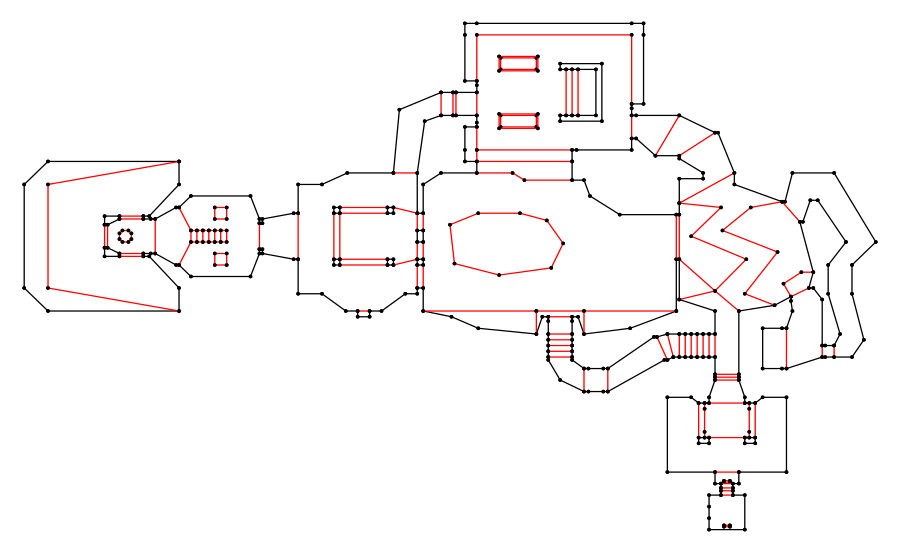
\includegraphics[width=\textwidth]{drawings/E1M1_lines.pdf}
\end{figure}
\par
The map as it is generated via the editor (DoomED) on NextStation.\\
\par
\begin{figure}[H]
\centering
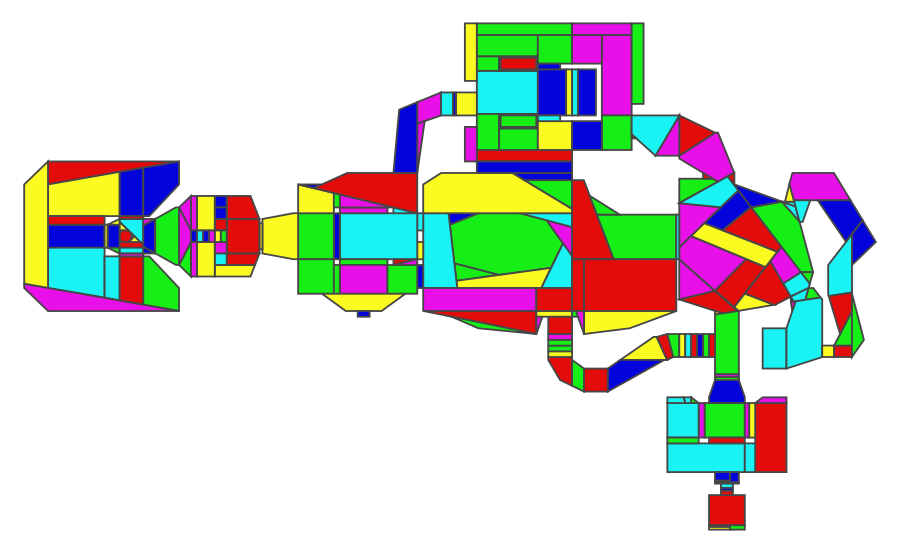
\includegraphics[width=\textwidth]{drawings/E1M1_fab.pdf}
\end{figure}
\par
Binary space partition. Slice all sectors into convex sub-spaces called subsectors.\\
\par
\begin{figure}[H]
\centering
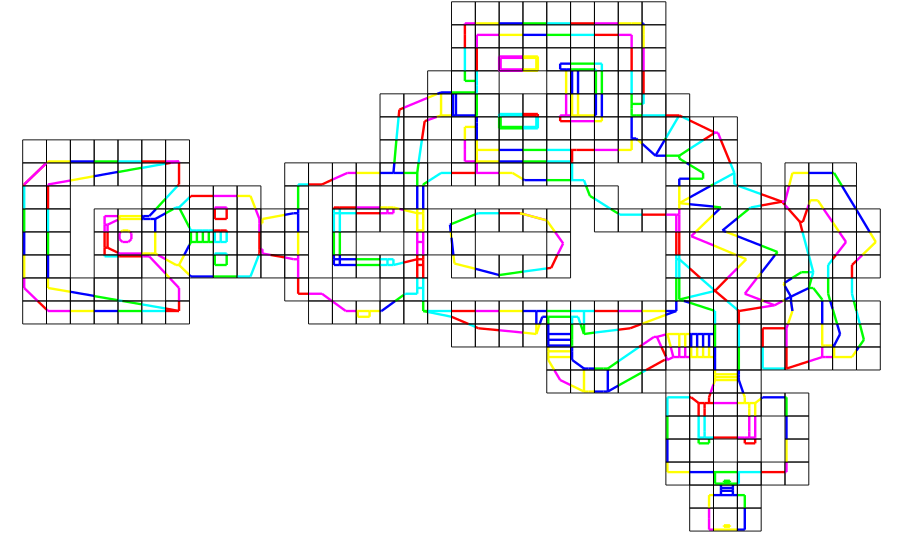
\includegraphics[width=\textwidth]{drawings/E1M1_blockmap.pdf}
\end{figure}
\par
Block based line index.\\
\par
\begin{figure}[H]
\centering
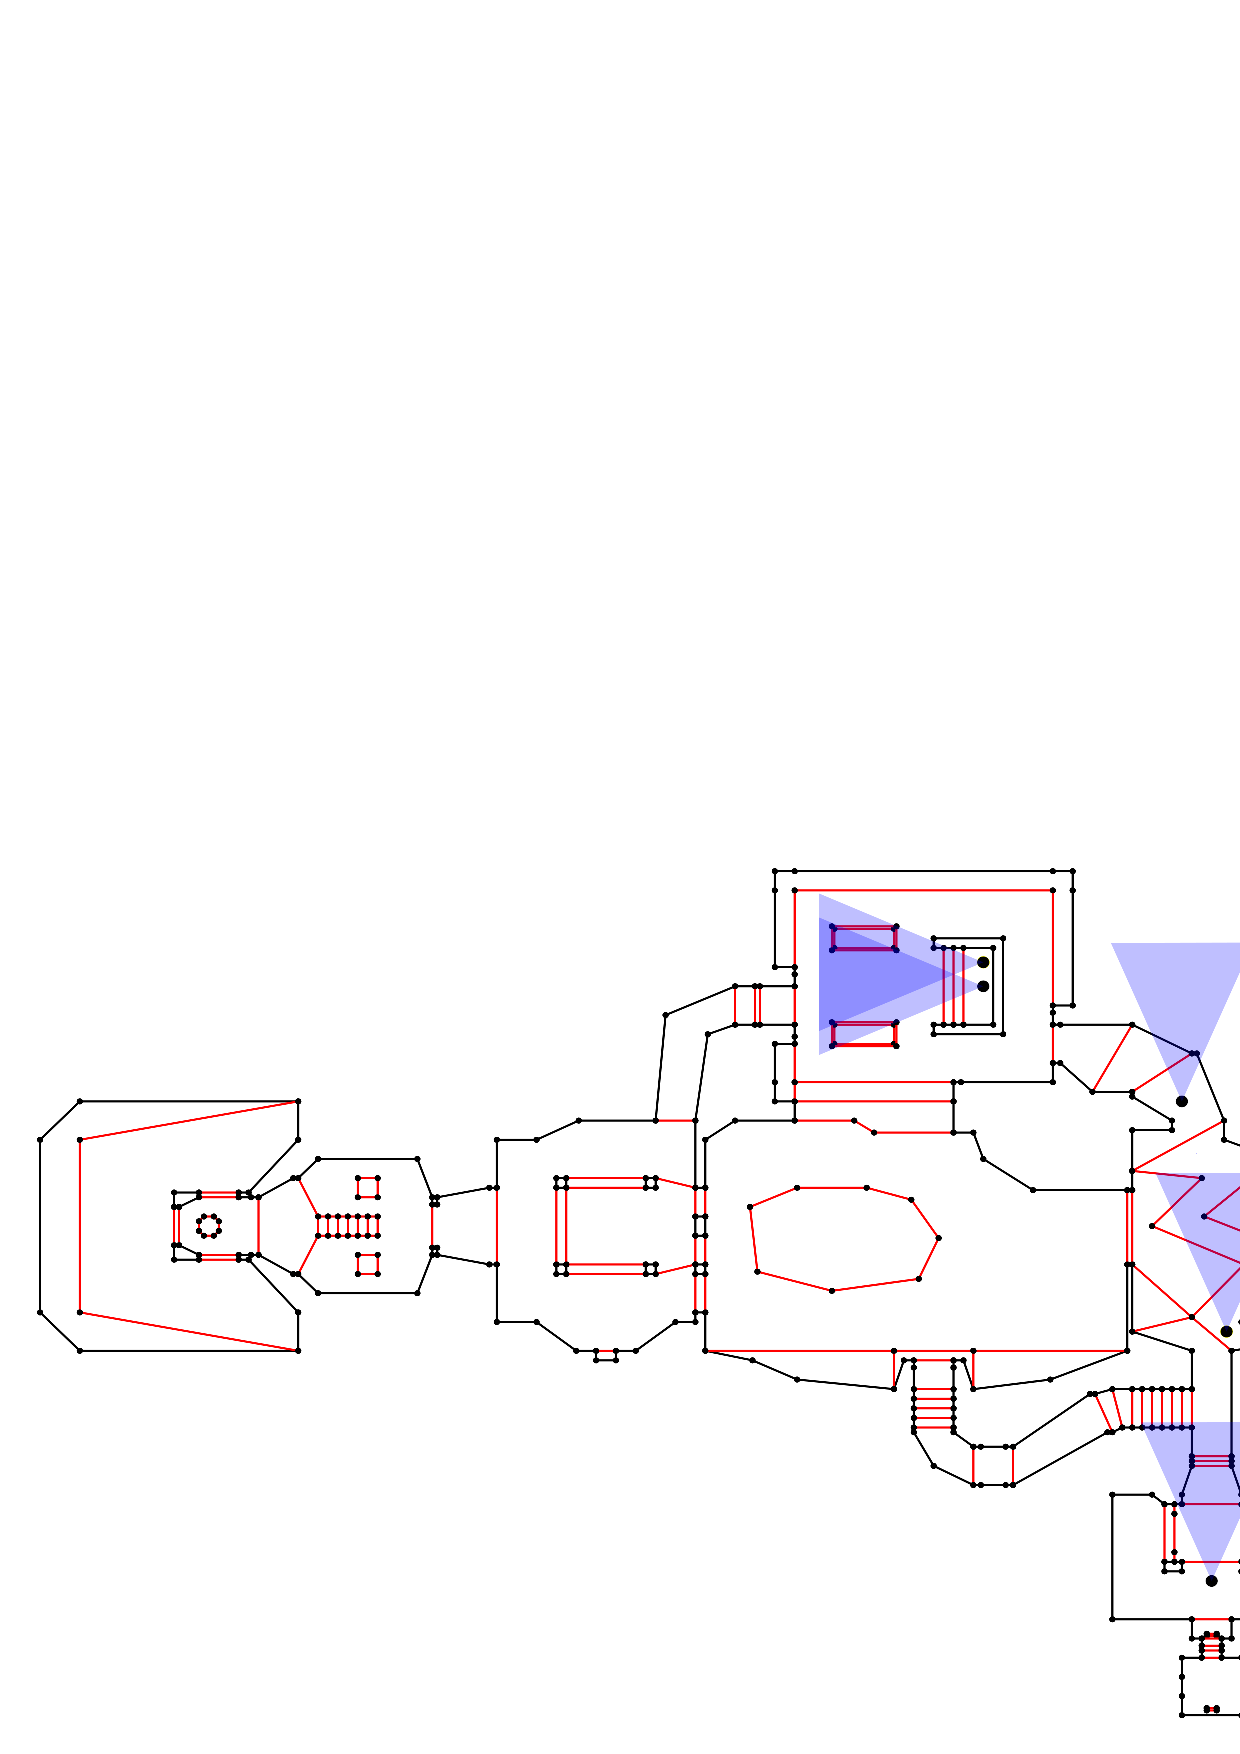
\includegraphics[width=\textwidth]{drawings/E1M1_sides.pdf}
\end{figure}
\par
Reject map based on enemies and monsters line of sight.\\


\pagebreak
\cfullimage{doombsp_compiling.png}{Building doombsp.}
\par
\cw{doombsp} generated several lumps and packaged them into a \cw{.wad} file\footnote{Explained on page XXX}.
\par
ARRAY OF LUMPS.
E1M1\\
THINGS\\
LINEDEFS\\
SIDEDEFS\\
VERTEXES\\
SEGS\\
SSECTORS\\
NODES\\
SECTORS\\
REJECT\\
BLOCKMAP\\
\par
\cfullimage{doombsp_run.png}{Running doombsp in debug mode show splitter selection.}
\par
